\documentclass{acm_proc_article-sp}
\usepackage{graphicx}
\usepackage{amsmath}
\usepackage{enumerate}
\usepackage{multirow}
\usepackage{epstopdf}
\usepackage{array}
\usepackage{CJK}
\usepackage{float}
\usepackage{subfigure}
\usepackage{algorithm}
\usepackage{algorithmicx}
\newcommand{\algorithmicbreak}{\textbf{break}}
\newcommand{\BREAK}{\State \algorithmicbreak}
\usepackage{algpseudocode}
\newtheorem{problem}{\textbf{Problem}}
\begin{document}

\title{Exploiting Publication Contents and Collaboration Networks for Collaborator Recommendation}
\subtitle{
%[Extended Abstract]
\titlenote{A full version of this paper is available as
\textit{Author's Guide to Preparing ACM SIG Proceedings Using
\LaTeX$2_\epsilon$\ and BibTeX} at
\texttt{www.acm.org/eaddress.htm}}}

\numberofauthors{8}

\author{
% 1st. author
\alignauthor
Ben Trovato\titlenote{Dr.~Trovato insisted his name be first.}\\
       \affaddr{Institute for Clarity in Documentation}\\
       \affaddr{1932 Wallamaloo Lane}\\
       \affaddr{Wallamaloo, New Zealand}\\
       \email{trovato@corporation.com}
% 2nd. author
\alignauthor
G.K.M. Tobin\titlenote{The secretary disavows
any knowledge of this author's actions.}\\
       \affaddr{Institute for Clarity in Documentation}\\
       \affaddr{P.O. Box 1212}\\
       \affaddr{Dublin, Ohio 43017-6221}\\
       \email{webmaster@marysville-ohio.com}
% 3rd. author
\alignauthor Lars Th{\o}rv{\"a}ld\titlenote{This author is the
one who did all the really hard work.}\\
       \affaddr{The Th{\o}rv{\"a}ld Group}\\
       \affaddr{1 Th{\o}rv{\"a}ld Circle}\\
       \affaddr{Hekla, Iceland}\\
       \email{larst@affiliation.org}
\and  % use '\and' if you need 'another row' of author names
% 4th. author
\alignauthor Lawrence P. Leipuner\\
       \affaddr{Brookhaven Laboratories}\\
       \affaddr{Brookhaven National Lab}\\
       \affaddr{P.O. Box 5000}\\
       \email{lleipuner@researchlabs.org}
% 5th. author
\alignauthor Sean Fogarty\\
       \affaddr{NASA Ames Research Center}\\
       \affaddr{Moffett Field}\\
       \affaddr{California 94035}\\
       \email{fogartys@amesres.org}
% 6th. author
\alignauthor Charles Palmer\\
       \affaddr{Palmer Research Laboratories}\\
       \affaddr{8600 Datapoint Drive}\\
       \affaddr{San Antonio, Texas 78229}\\
       \email{cpalmer@prl.com}
}

\additionalauthors{Additional authors: John Smith (The Th{\o}rv{\"a}ld Group,
email: {\texttt{jsmith@affiliation.org}}) and Julius P.~Kumquat
(The Kumquat Consortium, email: {\texttt{jpkumquat@consortium.net}}).}
\date{30 July 1999}

\maketitle
\begin{abstract}
Due to the expansion of academic research in diverse fields, the problem of finding relevant and potential collaborators has become cumbersome. In this work, we propose an academic collaboration recommendation model called CCRec. CCRec combines publication contents with collaboration networks to effectively generate academic collaboration recommendation for researchers. Using the DBLP data sets, we conduct benchmarking experiments to examine the performance of CCRec. Our preliminary experimental results show that CCRec outperforms other state-of-the-art methods especially in addressing the topic drift problems.
\end{abstract}

% A category with the (minimum) three required fields
\category{H.4}{Information Systems Applications}{Miscellaneous}
%A category including the fourth, optional field follows...
\category{D.2.8}{Software Engineering}{Metrics}[complexity measures, performance measures]

\terms{Theory}

\keywords{Collaboration recommendation, publication contents, collaboration networks, topic clustering, random walk.}

% =============================================================================
\section{Introduction}
% =============================================================================
Nowadays, with rapid development of Internet technology, the scale of Internet is beyond the imagination of people and Internet gradually becomes the main carrier of sharing information. Thus, how to obtain the useful one from vast information has become a complex task with the problem of information overload phenomena occurring. Therefore, recommender systems and techniques immensely help people by providing easier access to the specific resources they really need.

In academia, cooperation among researchers is of vital necessary. Studies show that researchers are usually prolific by well collaboration with collaborators. This is to say, the collaborator is a considerable factor well connected with the productivity of a scholar. So scholars tend to get acquainted with potential collaborators, especially the most valuable collaborators. In academic social networks, there has been a variety of methods proposed recommending collaborators who they have ever collaborated with or never.

In this context, previous studies have exploited mainly two aspects for academic collaboration recommendation, that is content-based and collaboration network-based methods respectively. Plenty of researches show that the traditional content-based method mostly focuses on the tags made by people, which can not completely stand for the research topic of the scholar. Thus, it would be imperative taking research field into account when recommending collaborators, particularly the personalized recommendation on account of various research fields. For the collaboration network-based method, there has been a suite of methods such as Random Walk algorithm, but rarely methods have ever integrated the content-based and collaboration network-based method. What's more, in view of the burdensome and embarrassing initial collaboration with unconnected researchers ever and the less value of already known collaborators, the unconnected researchers are more deserve to be recommended to seek more potential and valuable collaborators.

In this paper, we propose a novel hybrid model exploiting publication contents and collaboration networks for collaborator recommendation called CCRec. CCRec combines the content-based method and collaboration network-based method by synthesizing publication contents and collaboration networks. Because the publication contents are largely on behalf of the research field of a scholar, we can more precisely achieve the personalized recommendation according to their different kinds of research fields. We extract key words from publication contents of all researchers and divide these key words into several topics, then get a number of research fields corresponding to different researchers. For researchers tend to collaborate with those in the similar research field, thus in each topic there is a big collaboration network. Therefore, we explore all the collaboration networks in each research topic. With the publication contents and collaboration networks combined, CCRec greatly outperforms other traditional methods recommending totally new collaborators.

CCRec first uses topic clustering to partition the words from all the publications' titles into multiple domains. Then, CCRec computes the degree of interest (DoI) and the strength of influence (SoI) pertaining to each domain for each researcher. Finally, DoI and SoI are combined to form the feature vector for each researcher. By comparing the similarity of feature vector, CCRec provides a TopN collaboration recommendation list.

The remainder of the paper is structured as follows. Section 2 briefly presents the related work. We discuss the details of our model in section 3, which highlights the problem statement and the structure of the model. In section 4, we conduct a mass of experiments and analyzes the results. At last, section 5 concludes the paper.
% =============================================================================
\section{RELATED WORK}
% =============================================================================


% =============================================================================
\section{DESIGN OF CCRec}
% =============================================================================
Our proposed design scheme for CCRec is inspired by the reality and truth that a researcher usually desires to know other researchers who have similar research interests and strong influence in academia. As mentioned above, researchers often behave differently across multiple domains of interests. Such behaviors usually reveal academic features of different researchers in different domains. Besides, as a social-based model, the RWR model has been proved to be competent for calculating the rank score of node in social networks derived from the co-authorship \cite{li2014acrec}, researchers' strength of influence in specific domains can be well reflected by RWR. In this work, we adopt a content-based method to acquire multiple domains of interests. and use RWR to measure the researchers' strength of influence in different domains. After that, We use the feature vector to evaluate the similarity of researchers and then obtain the recommendation list. The detailed process is described bellow and the corresponding pseudo-code is illustrated in Algorithm 1. Figure 1 depicts the three components of CCRec.

%Initially,

%In this work, we proposed a content-based method to acquire multiple domains of interests. Furthermore, we define the SoI (Strength of Influence) to denote the %academic values (Rank Score) of researchers in different domains, which can be regarded as the elements of feature vector of researchers. Finally,we use the %feature vector to evaluate the similarity of researchers and then obtain the recommendation list.
%Topic clustering and researcher partition distribute researchers according to multiple domains.
\begin{figure}
\centering
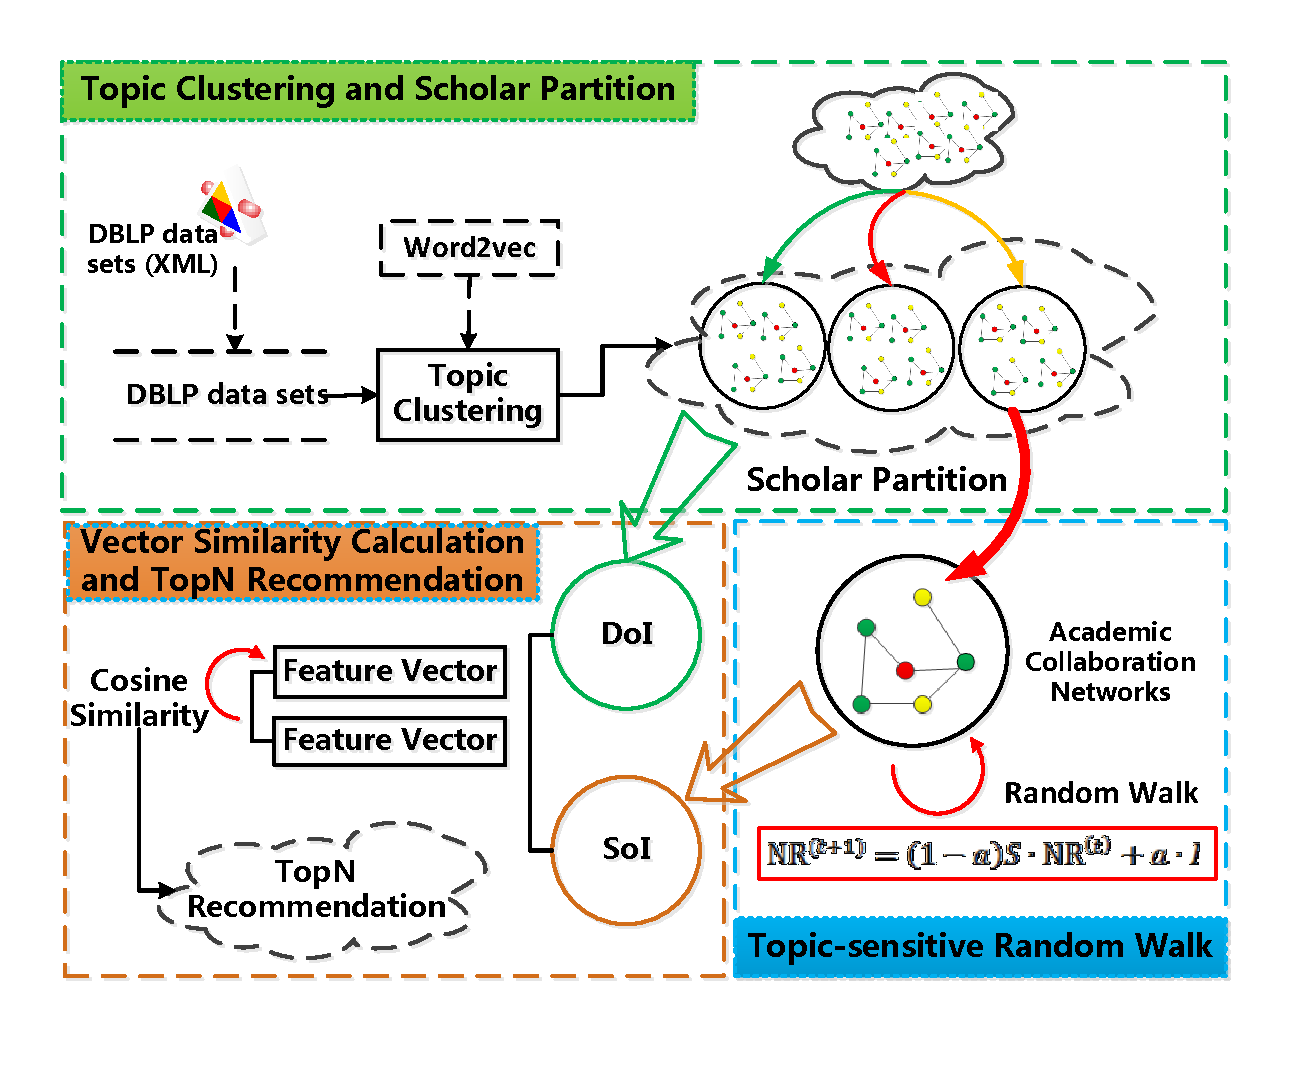
\includegraphics [width=3.4in]{Fig1.pdf}
\caption{The architecture diagram of CCRec model}
\end{figure}
\subsection{Topic Clustering and Researcher Partition}
% -----------------------------------------------------------------------------
It is a content-based method for topic clustering and researcher partition, which generates various domains and maps all researchers into these domains. In this work, we use a famous tool of NLP (Natural Language Processing), word2vec, which provides an efficient implementation of the continuous of \emph{bag-of-words} and \emph{skip-gram} architectures for computing vector representations of words. It takes a text corpus as input and produces the word vectors as output. The resulting word vector file can be used as features in many natural language processing and machine learning applications. The word vectors can be also used for deriving word classes from huge data sets. This is achieved by performing K-means clustering on top of the word vectors. The output is a vocabulary file with words and their corresponding class IDs. In case of CCRec model, the input data is a set of titles from all the papers created by each researcher. The titles are split in many sequential words. In addition,  there is a necessary to filter out some irrelevant words, e.g. "of","the", "and", etc. For extracting from titles, this set of preprocessed words can outline the core contents of papers, which are signified as valuable and reliable corpus to denote a variety of academic topics. With this English corpus,word2vec obtains various domains and cluster the word into the domains.

In addition, CCRec partitions researchers to particular domains with follows method. 1, Extract mesh terms from a researcher's publications. 2, Traverse all the terms and check the word vector. The model will tag the researcher to the particular domains which contains these domains. It should be emphasized that one researcher always belongs to several domains and there are also many researchers in one domain.

\subsection{Feature Vector Calculation}
% -----------------------------------------------------------------------------
As mentioned in section 2, in general, researchers devote to several adjacent domains. But in the case of attention and strength of influence in various domains, they are offering some biases. To measure the distribution of researchers' interest, we define the $SoI$ (Strength of Influence) to denote the academic values (Rank Score) of researchers in different domains, which can be regarded as the elements of feature vector of researchers. In case of one of the domains, there are numerous researchers with similar research interest. Their co-author relationships can be modeled by a network. Thus, there are many co-author networks corresponding to different domains. The $SoI$ is measured by RWR model based on the co-author networks. The core equation of the RWR model is shown below:
\begin{equation}
R_{d}^{(t+1)}=\alpha \mathbf{S}R_{d}^{(t)}+(1-\alpha)q
\end{equation}
where $R_{d}$ represents the rank score vector of all researchers in domain $d$, $q$ is the initial vector $R^0$, and $\alpha$ denotes the damping coefficient. RWR is an iterative process. After limited iterations, the vector $R$ will be convergent. In this scenario, $SoI_{s}=R_{d,s}$. That is, the final value of the vector item $R_{d,s}$ is the $SoI$ of researcher $s$.

In addition, with the help of RWR, The $SoI$s in various domains are quantified for each researcher. To measure researchers academic feature, we define the vector $F$ with $SoI$.

\subsection{Collaboration Recommendation by Feature Vector Similarity}
% -----------------------------------------------------------------------------
CCRec recommend collaborators for researchers based on their similarities. To measure the academic features similarity of researchers, we borrow a standard method, \emph{cosine similarity} (CS). CS is employed to define the similarity between two users $s_{1}$ and $s_{2}$ based on their feature vectors $F_{s_{1}}$ and $F_{s_{2}}$.
\begin{equation}
Sim(s_{1},s_{2})=\frac{\sum_{i=1}^{n}(F_{s_{1},i}*F_{s_{2},i})}{\sqrt{\sum_{i=1}^{n}F_{s_{1},i}^2}*\sqrt{\sum_{i=1}^{n}F_{s_{2},i}^2}}
\end{equation}
Finally, we consider that researchers with high similarities have common interest, they should be recommended to each other as potential academic collaborators. Hence, CCRec provide a TopN recommendation list for each researcher.

% =============================================================================
\section{Evaluation and Analysis}
% =============================================================================
We conduct various experiments using data from DBLP \cite{Ley:DBLP}, a computer science bibliography website hosted at University Trier. We extracted the subsets of the entire data using the required information, which are all in the field of data mining involving 34 journals and 49 conferences. The data was modeled by an academic social network, which contains 59659 nodes (authors) and 90282 edges (coauthor relations). We divided the data set into two parts: the data before year 2011 as a training set, and others as a testing set.To evaluate the performance of CCRec model, we use three metrics widely used in the recommender systems, \emph{Precision}, \emph{Recall} and \emph{F1} \cite{shani2011evaluating}.

All experiments were performed on a 64-bit Linux-based operation system, Ubuntu 12.04 with a 4-duo and 32GHz Intel CPU, 4-G Bytes memory. All the programs are implemented with Python.
\begin{figure*}
\centering
\subfigure[Precision]{
\label{fig:2-a}
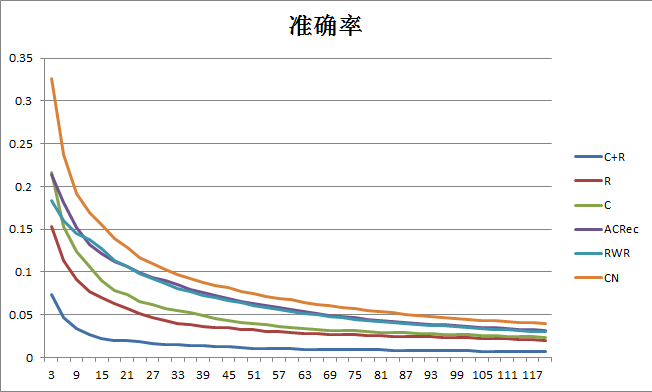
\includegraphics[width=0.32\textwidth]{Fig2-a.png}}
\subfigure[Recall Rate]{
\label{fig:2-b}
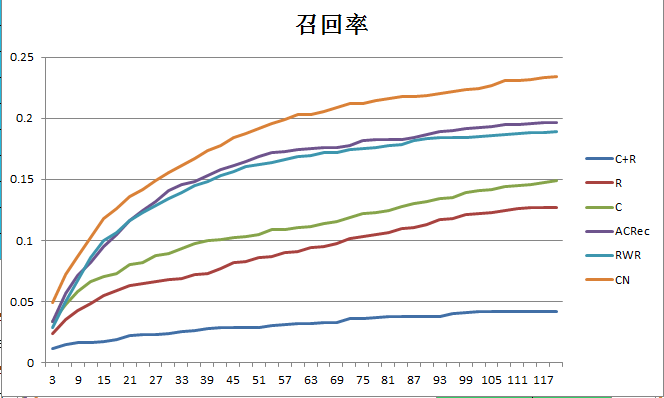
\includegraphics[width=0.32\textwidth]{Fig2-b.png}}
\subfigure[F1]{
\label{fig:2-c}
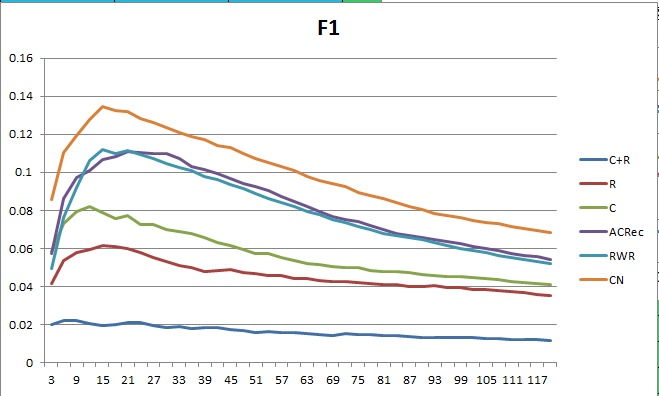
\includegraphics[width=0.32\textwidth]{Fig2-c.png}}
\caption{Performance of CCRec, RWRec and CNRec}
\label{fig:5}       % Give a unique label
\end{figure*}
\begin{figure*}
\centering
\subfigure[Precision]{
\label{fig:3-a}
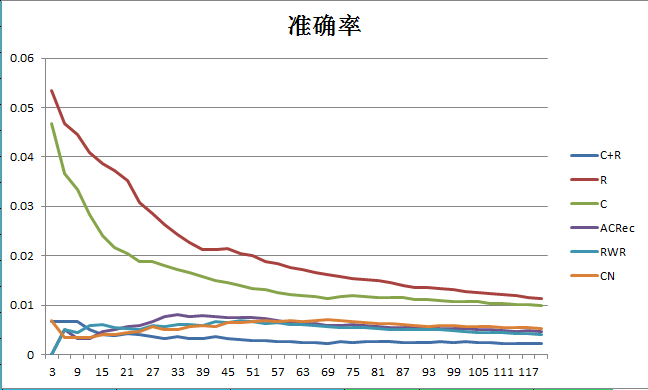
\includegraphics[width=0.32\textwidth]{Fig3-a.png}}
\subfigure[Recall Rate]{
\label{fig:3-b}
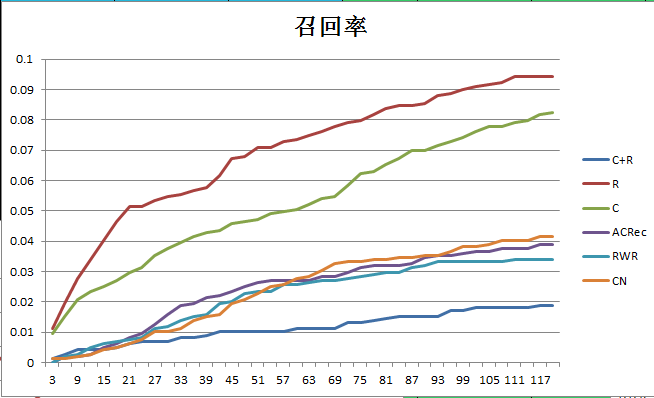
\includegraphics[width=0.32\textwidth]{Fig3-b.png}}
\subfigure[F1]{
\label{fig:3-c}
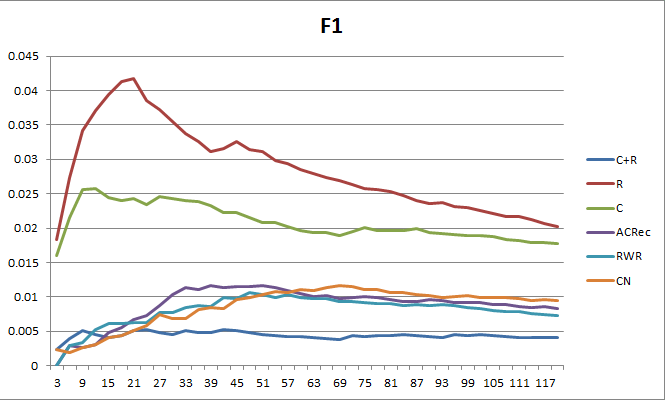
\includegraphics[width=0.32\textwidth]{Fig3-c.png}}
\caption{Performance of CCRec, RWRec and CNRec}
\label{fig:5}       % Give a unique label
\end{figure*}

Using a subset of DBLP dataset relevant to data mining, we embarked on benchmarking experiments to evaluate the performance of CCRec. We took the year 2011 as the partition time of training and testing sets. To evaluate our model in a better way, we compared CCRec with the two following approaches. RWRec: a random walk recommendation model based on collaboration networks. CNRec: a common neighbors based recommendation model \cite{lopes2010collaboration}. We adopted three metrics to evaluate the performance of CCRec: precision, recall rate and F1. We recommend the new collaborators who never cooperated with the target researcher, because the new collaborators are more meaningful and practical in academia.

Figure 2 shows the performance of CCRec, RWRec and CNRec in terms of precision, recall rate and F1 with the number of recommended collaborators increasing. It can be observed that CCRec significantly outperforms RWRec and CNRec all the time in these three metrics. CCRec shows a downtrend for precision and an uptrend for recall rate. In the case of F1, it reaches the peak 6.598\% when recommending 18 researchers.

In a nutshell, CCRec outperforms RWRec and CNRec with higher precision, recall rate and F1. This is because CCRec combines publication contents and collaboration networks which has a distinct advantage in recommending new collaborators.

% =============================================================================
\section{Conclusions}
% =============================================================================
The conclusions we reach are: 1) CCRec outperforms RWRec and CNRec in precision, recall rate and F1 integrating publication contents with academic collaboration networks. 2) With topic clustering, the problem of topic drift has been well solved.

Our research on CCRec reveals that the combination of information regarding publication contents and collaboration networks of researchers can improve the generation of effective academic collaborations.

\section{Acknowledgments}

\bibliographystyle{abbrv}
\bibliography{CCRec-Full}
\balancecolumns

\end{document}
